\vspace{10pt}
\section{Analysis of Design Constraints}\label{sec:wr}
\subsection{Overview}
As shown in Figure.~\ref{fig:modeling}, in order to write or read the cross point array, the external voltages should be applied at the end of the word line and the bit line. Although there are several potential read/write schemes can be used to program the memory array, it is difficult to point out which schemes is the most proper choice under given design constraints of area/energy/reliability. Therefore, in this section, studies on different operation schemes and present are conducted. The results of this study can be very useful to guide the design of the cross point array. Since it is impossible to consider all of the data pattern stored in the array, in this work, the best and worst cases are studied.

Table~\ref{table:parameter} shows the circuit parameter of our baseline design. The data is consistent to the recently published studies on ReRAM~\cite{crossbar_TED_2010}\cite{memristor:Cong}.

\begin{table}[!b]
  \centering
  \scriptsize
    \scriptsize
  \caption{Parameters of the baseline Cross Point Array}\label{table:parameter}
  \vspace{-5pt}
%  \begin{tabular}{|cccccp{3.5cm}|}
  \begin{tabular}{c|c|c}
    \hline    \hline
    % after \\: \hline or \cline{col1-col2} \cline{col3-col4} ...
    \textbf{Metric} & \textbf{Description} & \textbf{Values} \\
    \hline
    \textbf{$S_{cell}$} & Cell Size & \textbf{$4F^2$} \\
    \textbf{$R_l$} &  Interconnection Resistance&\textbf{$1.25\Omega$} \\
    \textbf{$R_s$} &  Resistance of SA&\textbf{$100\Omega$} \\
    \textbf{$V_{RESET}$} & Threshold voltage for RESET&\textbf{$2.0V$} \\
    \textbf{$V_{SET}$} & Threshold voltage for SET&\textbf{$-2.0V$} \\
    \textbf{$V_{READ}$} & Read Voltage of Cell&\textbf{$0.5V$} \\
    \textbf{$R_{off}$} & HRS Resistance &\textbf{$500K\Omega$} \\
    \textbf{$R_{on}$} & LRS Resistance &\textbf{$10K\Omega$} \\
    \textbf{$V_{W}(R)$} & Word Line Voltage during Read &\textbf{$\pm 1V ???$} \\
    \textbf{$V_{W}(W)$} & Word Line Voltage during Write  &\textbf{$0 / 2V$} \\
    \textbf{$V_{W}(H)$} & Half Selected Word Line Voltage &\textbf{$1V$} \\
    \textbf{$V_{B}(R)$} & Bit Line Voltage during Read  &\textbf{$10K\Omega ????$} \\
    \textbf{$V_{B}(W)$} & Bit Line Voltage during Write  &\textbf{$0 / 2V$} \\
    \textbf{$V_{B}(H)$} & Half Selected Bit Line Voltage &\textbf{$1V$} \\
    \textbf{$M$} & Number of Word Line &\textbf{$64$} \\
    \textbf{$N$} & Number of Bit Line &\textbf{$64$} \\

    \hline
  \end{tabular}
  \vspace{-10pt}
\end{table}

Considering that program schemes for write and read operation are different and the the requirement for write and read are also dissimilar, in the following section we carefully study the write and read operation separately. And then the results are combined together to provide a design methodology for the cross point array.

\subsection{Write Operation}
To write a ReRAM cell, a external voltage is required to applied across the cell for a certain duration. Intuitively, there are four possible schemes for the write operation:
\begin{enumerate}
  \item According the location of the target cell, activate one word line and one bit line and leave all of the other lines floating (FWFB shemes).
  \item Activate the targeted word line and bit line. Left all the other word line floating and half bias the other bit line (FWHB shemes).
  \item In contrast with the scheme 2, activate the targeted word line and bit line. Left all the other bit line floating and half bias the other wold line (HWFB shemes).
  \item Activate the targeted word line and bit line. Half bias all of the other bit line (HWHB shemes).
\end{enumerate}

In the ideal condition, all of these four schemes can provide enough voltage drop across the specified cell. However, the realistic circuit is not perfect and the electronic behavior of the array will deviate from the ideal scenario. In this section, the reliability, energy consumption and area overhead for the four write schemes based on our basic circuit parameter as shown in Table.~\ref{table:parameter}. Then the sensitivities of these schemes to resistance values of HRS and LRS ReRAM cell, and interconnect wire are studied.

\vspace{10pt}
\textbf{Reliable Write Operation.}
\vspace{8pt}

The most important issue for the write operation is the reliability concern. A reliable write operation can be defined as: switching the selected cells into required states without disturbing the states of unselected cells. Therefore, there exist two potential write error:
\textbf{write failure} and \textbf{write disturbance}. All of the write schemes should at least meet the reliability requirement at the worst case. On the other word, the designer should make sure there is not any write failure and write failure disturbance occur even in the worst case. 
First of all, we will show the inherent problem of FWFB scheme, which may result in severs write disturbance. The worse case scenario for FWFB write disturbance can be defined as: all of unselected cells in the activated word line (or all of unselected cells in the activated bit line) are at HRS and other cells are in LRS. In this case, as shown in Figure. 
\begin{figure}%[!hb]
\centering
  % Requires \usepackage{graphicx}
  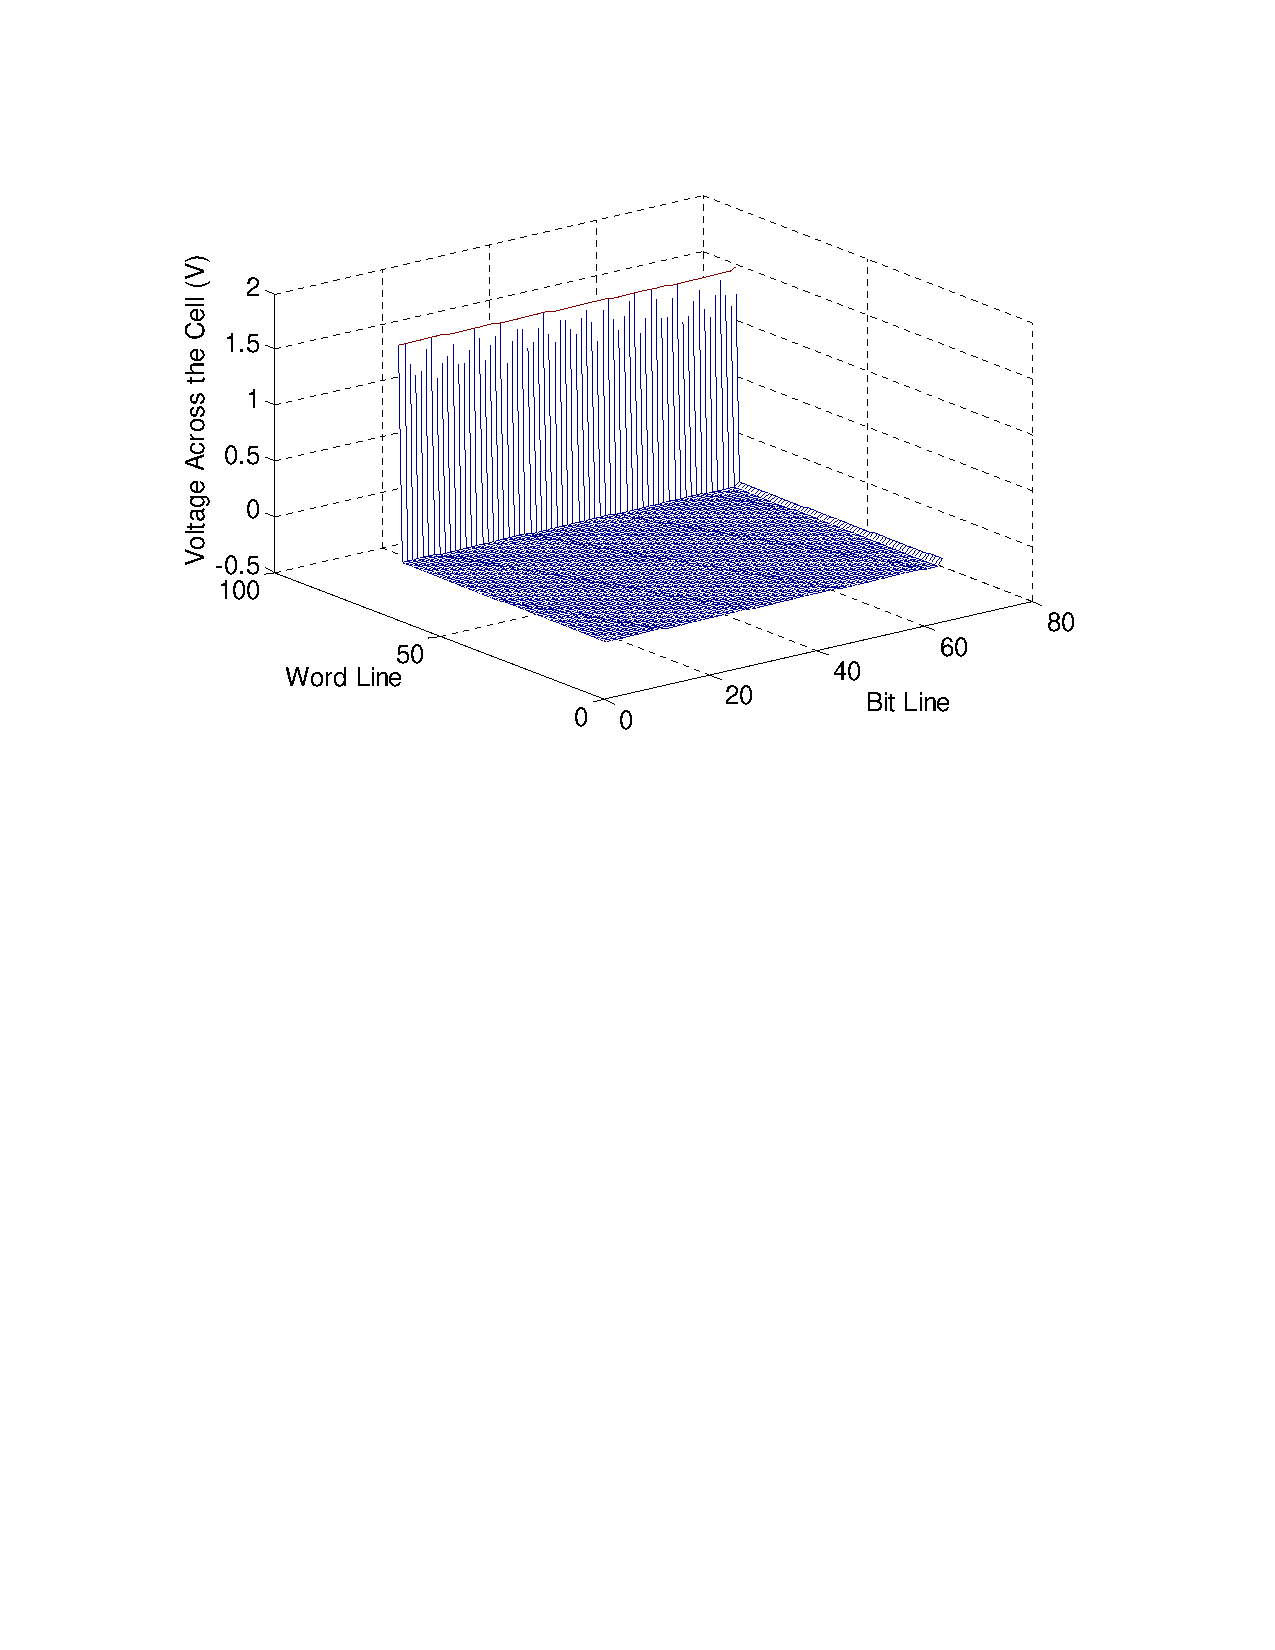
\includegraphics[width=0.45\textwidth]{./figures/FWFB.pdf}\\
  \caption{Write Disturbance for FWFB Schemes.}\label{fig:FWFR}
\end{figure}



  
The worst case scenario of write disturbance for each each schemes can be 




1. Only consider the one-side scheme
Consider 1/2 1/3 and floating?
Energy Issue? Define Energy Efficient Parameter?
Reliable Issue: Any possibility of write disturbance




2. Present the voltage drop problem
Reliability Issue

3. Two Way Scheme

\subsection{Read Operation} 